\block{Diagrammatic representation of a queue}{
    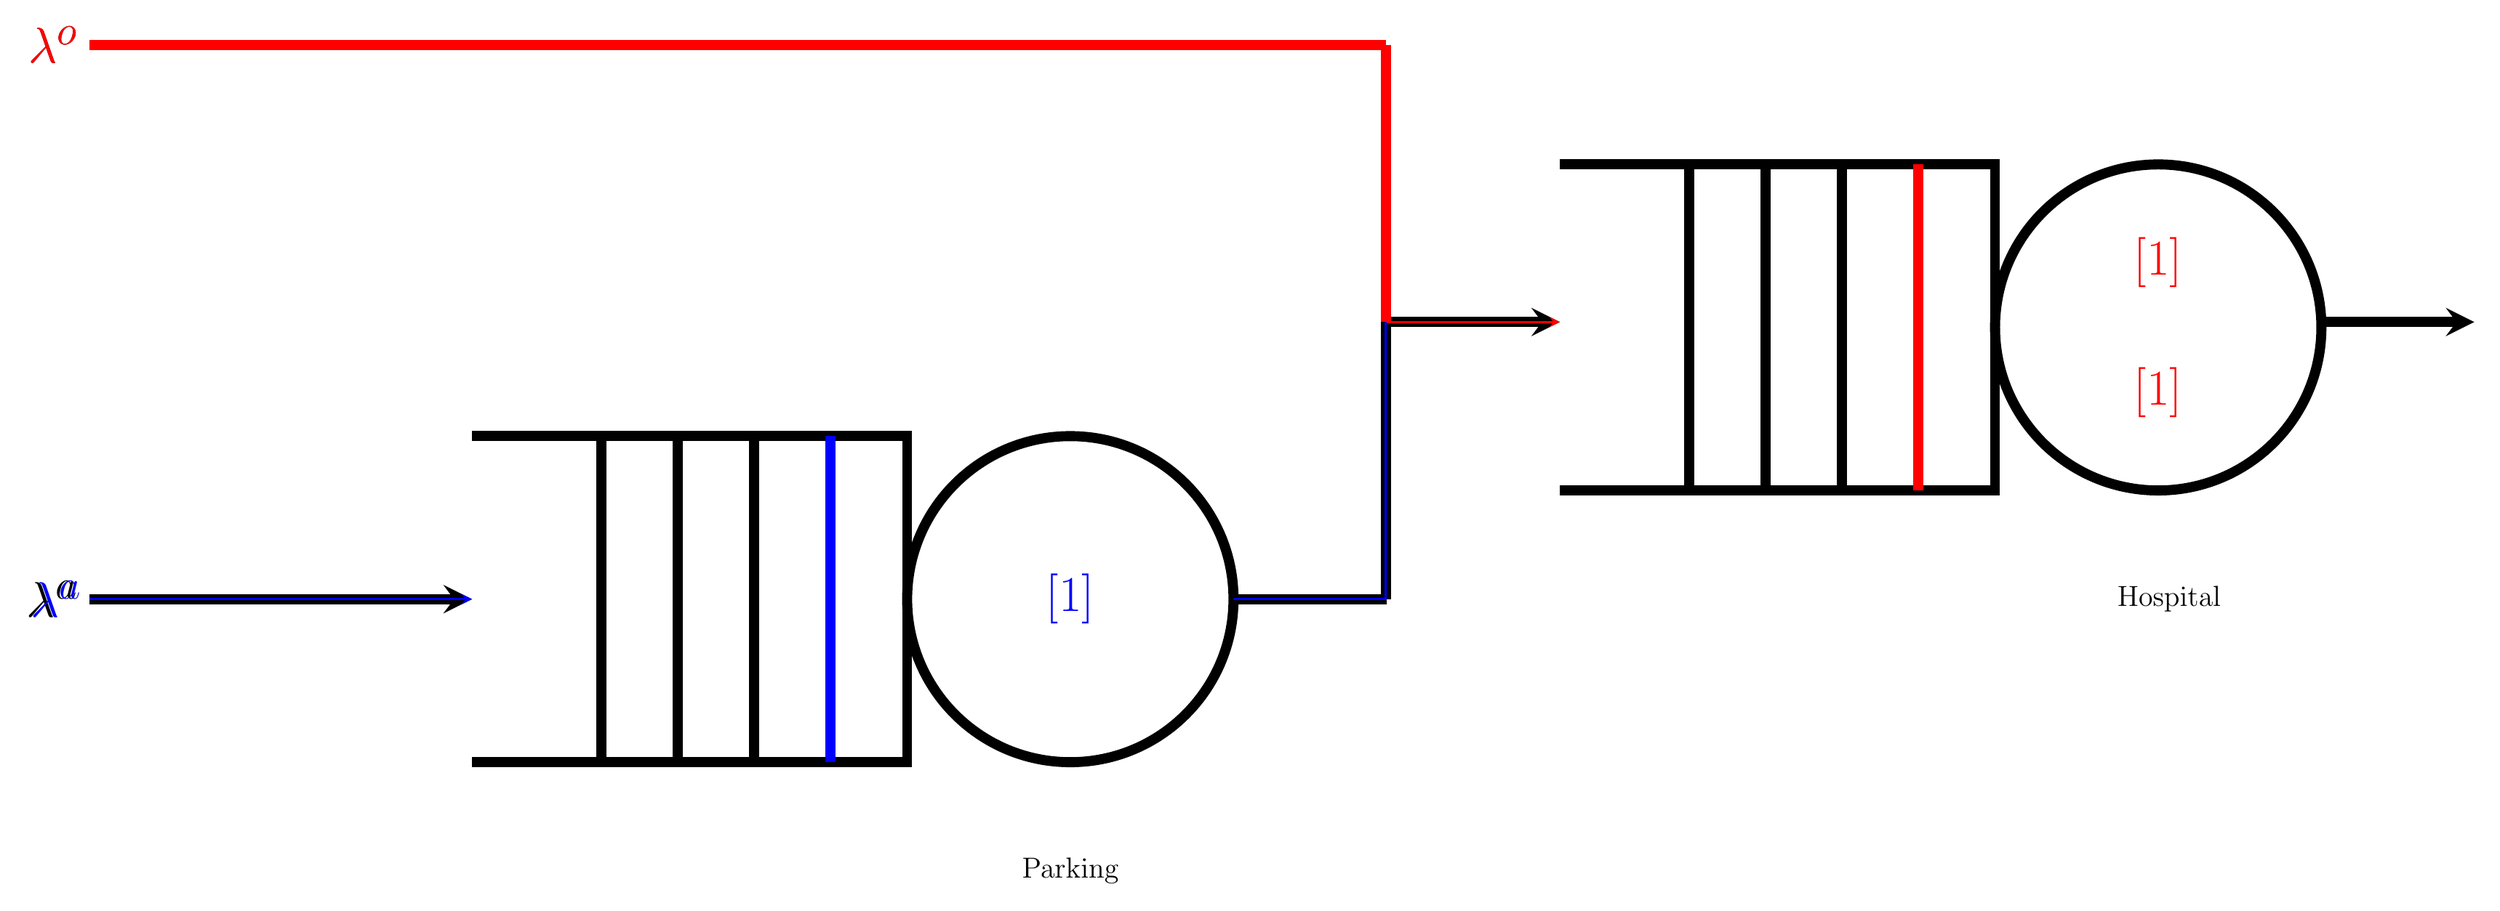
\begin{tikzpicture}[>=stealth, scale=3.8, font=\Huge],
        % the rectangle with vertical rules (Queue 1)
        \draw[line width=5pt] (0,0) -- ++(2cm,0) -- ++(0,-1.5cm) -- ++(-2cm,0);
        \foreach \i in {1,...,4}
        \draw[line width=5pt] (2cm-\i*10pt,0) -- +(0,-1.5cm);
        
        % the circle (Queue 1)
        \draw[line width=5pt] (2.75,-0.75cm) circle [radius=0.75cm];

        % the rectangle with vertical rules (Queue 2)
        \draw[line width=5pt] (5,1.25) -- ++(2cm,0) -- ++(0,-1.5cm) -- ++(-2cm,0);
        \foreach \i in {1,...,4}
        \draw[line width=5pt] (7cm-\i*10pt,1.25) -- +(0,-1.5cm);

        % the circle (Queue 2)
        \draw[line width=5pt] (7.75,0.5) circle [radius=0.75cm];

        % the arrows and labels (Queue 1+2)
        \draw[->, line width=5pt] (8.5,0.525) -- +(20pt,0);
        \node[align=center] at (1cm,-2cm) {};
        \node[align=center] at (2.75cm,-2cm) {\Large{Parking}};
        \node[align=center] at (6cm,-0.75cm) {};
        \node[align=center] at (7.8cm,-0.75cm) {\Large{Hospital}};
        
        % Ambulance lines
        \draw[<-, line width=5pt] (0,-0.75) -- +(-50pt,0) node[left] {\Huge{\(\lambda^a \)}};
        \draw[-, line width=5pt] (3.5,-0.75) -- +(20pt,0);
        \draw[line width=5pt] (4.2, 0.525) -- (4.2, -0.75);

        % Others lines
        \draw[line width=5pt] (4.2, 1.8) -- +(-169.5pt,0) node[left] {\Huge{\( \lambda^o \)}};
        \draw[line width=5pt] (4.2, 1.8) -- (4.2, 0.525);
        \draw[->, line width=5pt] (4.2, 0.525) -- (5, 0.525);  

        % Stick figures
        \node[draw=none, red] at (7.75,0.8) {\Huge{\Strichmaxerl[1]}};
        \node[draw=none, red] at (7.75,0.2) {\Huge{\Strichmaxerl[1]}};
        \draw[red, very thick, line width=5pt] (4.2, 1.8) -- +(-169.5pt,0) node[left] {\Huge{\(\lambda^o\)}};
        \draw[red, very thick, line width=5pt] (4.2, 1.8) -- (4.2, 0.525);
        \draw[->, line width=5pt, red, very thick] (4.2, 0.525) -- (5, 0.525);
        \draw[-, line width=5pt, blue, very thick] (3.5,-0.75) -- +(20pt,0);
        \draw[blue, very thick] (4.2, 0.525) -- (4.2, -0.75);
        \draw[<-, line width=5pt, blue, very thick] (0,-0.75) -- +(-50pt,0) node[left] {\Huge{\(\lambda^a\)}};
        \node[draw=none, blue] at (2.75,-0.75) {\Huge{\Strichmaxerl[1]}};
        \draw[blue, very thick, line width=5pt] (2cm-10pt,0) -- +(0,-1.5cm);
        \draw[red, very thick, line width=5pt] (7cm-10pt,1.25) -- +(0,-1.5cm);
    \end{tikzpicture}
}